\documentclass[11pt,a4paper]{article}

\usepackage[margin=23mm]{geometry}
\usepackage[T1]{fontenc}
\usepackage{lmodern}
\usepackage{microtype}
\usepackage{amsmath,amssymb,mathtools}
\usepackage{booktabs,longtable,tabularx,array}
\usepackage{graphicx}
\usepackage{float}
\usepackage{xcolor}
\usepackage{enumitem}
\usepackage{needspace}
\usepackage{fancyhdr}
\usepackage[hidelinks]{hyperref}
\usepackage{xurl}

\graphicspath{{figures/}}
\setlength{\parindent}{0pt}
\setlength{\parskip}{5pt}
\setlist{nosep,leftmargin=*}
\setcounter{tocdepth}{2}

\definecolor{methodblue}{HTML}{155A91}
\definecolor{methodorange}{HTML}{C65D16}
\definecolor{lightorange}{HTML}{FFF4EA}

\pagestyle{fancy}
\fancyhf{}
\lhead{\small Original Hybrid SPECTRA-Siam Methodology}
\rhead{\small Implementation-aligned specification}
\cfoot{\thepage}
\renewcommand{\headrulewidth}{0.4pt}
\fancypagestyle{plain}{%
  \fancyhf{}%
  \lhead{\small Original Hybrid SPECTRA-Siam Methodology}%
  \rhead{\small Implementation-aligned specification}%
  \cfoot{\thepage}%
  \renewcommand{\headrulewidth}{0.4pt}%
}

\newcommand{\method}{\textsc{Spectra-Siam}}
\newcommand{\R}{\mathbb{R}}
\newcommand{\concat}{\mathbin{\Vert}}
\newcommand{\softmax}{\operatorname{softmax}}
\newcommand{\sigmoid}{\operatorname{sigmoid}}
\newcommand{\LN}{\operatorname{LN}}
\newcommand{\Norm}{\operatorname{Normalize}_{2}}
\newcommand{\sym}{\operatorname{Sym}}
\newcommand{\GELU}{\operatorname{GELU}}
\newcommand{\mean}{\operatorname{mean}}

\title{\vspace{-12mm}\method{}\\[2mm]
\Large Original Hybrid Methodology\\[1mm]
\large Canonical, Lexical, Latent-Node, and Multi-Scale Spectral Fusion}
\author{Implementation-aligned technical specification}
\date{Architecture state before the spectral-only readout revision}

\begin{document}
\maketitle
\thispagestyle{empty}

\begin{abstract}
This document specifies the original hybrid \method{} architecture for semantic
code-clone detection. It deliberately describes the implementation state before
the later eigenvalue-only readout revision. The original model did not use a
single spectral feature family in isolation. It learned a latent program graph,
constructed a 152-dimensional multi-scale spectral descriptor, pooled the learned
latent-node states, fused the spectral and latent representations, and optionally
added a separate source-lexical residual. Canonical node categories and bounded
node-label lexical features also entered before graph induction. They could
therefore influence the learned graph, while simultaneously reaching the
prediction through non-eigenvalue paths. The complete data flow, dimensions,
trainable quantities, loss terms, gradient paths, and fusion points are stated
explicitly.
\end{abstract}

\begin{center}
\fcolorbox{methodorange}{lightorange}{%
\begin{minipage}{0.91\linewidth}
\textbf{Scope boundary.}
Every equation and architectural claim in this note refers to the original
\texttt{readout\_mode = "hybrid"} implementation. The later eigenvalue-only
configuration is not presented as the method here.
\end{minipage}}
\end{center}

\tableofcontents
\clearpage

\section{Problem definition and complete pipeline}

Given two code fragments $c_i$ and $c_j$, the model predicts
$y_{ij}\in\{0,1\}$, where one denotes a semantic clone. A shared encoder
$F_\Theta$ maps each fragment to a normalized code embedding
$\phi(c)\in\R^{256}$:
\begin{equation}
o_{ij}=C_\Psi\!\left(
\phi_i\concat\phi_j\concat|\phi_i-\phi_j|
\concat(\phi_i\odot\phi_j)\concat\cos(\phi_i,\phi_j)
\right),
\qquad
\widehat y_{ij}=\sigmoid(o_{ij}).
\end{equation}
The two branches share all parameters.

The original encoder is a hybrid pipeline:
\begin{equation}
\begin{aligned}
c
&\longrightarrow
\{A_{\rm in}^{(r)},\,\kappa_v,\,\ell_v,\,q(c)\}\\
&\longrightarrow H^{(0)}
\longrightarrow H
\longrightarrow (P,Z,A_\Theta)
\longrightarrow \bigl(s_\Theta,\bar z\bigr)\\
&\longrightarrow \phi_{\rm graph}
\longrightarrow \phi.
\end{aligned}
\end{equation}
Here $s_\Theta$ is the multi-scale spectral descriptor, $\bar z$ is the pooled
latent-node representation, and $q(c)$ is the optional 96-slot source-lexical
sketch. The graph embedding $\phi_{\rm graph}$ fuses $s_\Theta$ and $\bar z$.
When enabled, $q(c)$ is added afterward as a direct residual.

\begin{figure}[H]
\centering
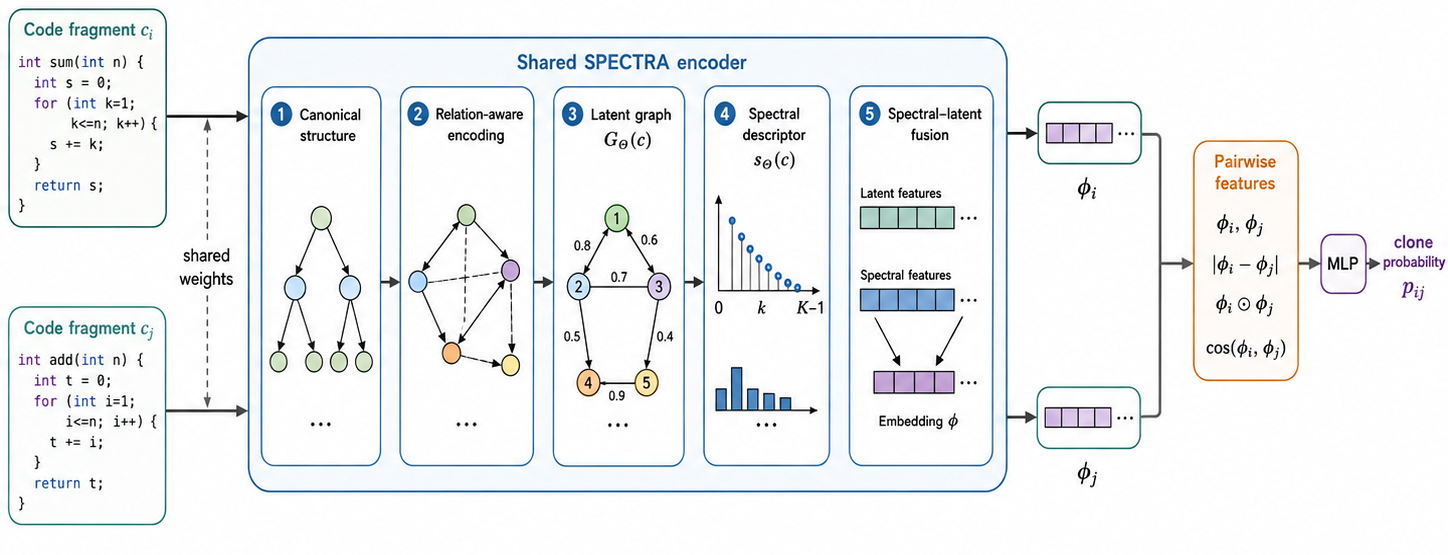
\includegraphics[width=\linewidth]{main_fig.png}
\caption{The original shared hybrid encoder. Stage 5 explicitly fuses spectral
features with pooled latent-node features. The optional source-lexical residual
is applied after the embedding shown in this figure.}
\label{fig:overview}
\end{figure}

\section{Notation and implementation dimensions}

\begin{table}[H]
\centering
\small
\begin{tabularx}{\linewidth}{@{}lclX@{}}
\toprule
Quantity & Symbol & Size & Meaning \\
\midrule
Retained input nodes & $n$ & $\leq256$ & Padded/truncated observed program graph \\
Hidden dimension & $d$ & $256$ & Node, latent-node, and code embedding width \\
Canonical vocabulary & $V_c$ & $25$ & Padding plus 24 normalized categories \\
Lexical hash vocabulary & $V_\ell$ & $4096$ & Padding plus stable hash buckets \\
Node lexical slots & $r$ & $4$ & Hashed features retained per input node \\
Source lexical slots & $r_s$ & $96$ & Optional whole-source lexical sketch \\
Observed relations & $R_{\rm in}$ & $1$ or $2$ & AST, or AST+DDG when node IDs align \\
Graph encoder layers & $L_g$ & $2$ & Relation-aware message-passing layers \\
Latent nodes & $m$ & $32$ & Fixed-size learned graph per program \\
Slot iterations & $T_s$ & $3$ & Iterative latent-node induction \\
Affinity heads & $H_a$ & $4$ & Multi-head latent adjacency scoring \\
Latent refinement layers & $L_z$ & $2$ & Message passing on learned adjacency \\
Density features & $J$ & $32$ & Smooth eigenvalue histogram \\
Heat features & $Q$ & $24$ & Heat traces at logarithmic scales \\
Chebyshev bands/signals & $B,S$ & $12,8$ & $96$ graph-signal energy features \\
Spectral descriptor & $d_s$ & $152$ & $32+24+12\times8$ \\
Pair feature & $d_p$ & $1025$ & $4d+1$ \\
\bottomrule
\end{tabularx}
\caption{Canonical dimensions of the original hybrid implementation.}
\end{table}

\section{Deterministic program representation}

\subsection{Observed graph}

Each fragment is parsed into an observed program graph. The data loader retains
at most 256 nodes and stores one binary adjacency matrix per permitted relation:
\begin{equation}
A_{\rm in}^{(r)}\in\{0,1\}^{n\times n},
\qquad r\in\mathcal R.
\end{equation}
The ordinary audited single-language setting uses AST and DDG. A setting in
which DDG and AST do not share a reliable node namespace uses AST only. The
sequential fallback relation exists in the serialized batch but is disabled in
the reported method configuration.

The observed graph is not itself the final graph used for spectral extraction.
It supplies structural messages and a projected prior for a learned 32-node
weighted graph.

\subsection{Canonical node categories}

Parser-specific node types are mapped deterministically to 24 normalized
categories. Zero is padding. The categories cover control flow, declarations,
operators, expressions, literals, structural blocks, identifier context, type
metadata, and an unknown category. The result for node $v$ is an integer
$\kappa_v\in\{0,\ldots,24\}$.

The integer is not a node-specific learned embedding. It indexes a shared
trainable table
\begin{equation}
E_{\rm can}\in\R^{25\times256}.
\end{equation}
All nodes with the same canonical ID retrieve the same initial canonical vector;
their contextual states diverge after graph message passing.

\subsection{Node-label lexical sketch}

The available node label is HTML-decoded, split at punctuation and camel-case
boundaries, lower-cased, and normalized for numeric, Boolean, and null-like
tokens. Short character trigrams from the first subtokens are also considered.
At most four features are retained and mapped by a stable BLAKE2-based hash:
\begin{equation}
\ell_v=(\ell_{v1},\ldots,\ell_{v4}),
\qquad \ell_{vq}\in\{0,\ldots,4095\}.
\end{equation}
No vocabulary is fitted on the training split. Numeric line labels are ignored.
These IDs index the shared table
\begin{equation}
E_{\rm lex}\in\R^{4096\times256}.
\end{equation}

\subsection{Whole-source lexical sketch}

The lexical-augmented configuration additionally tokenizes the source text into
identifiers, numbers, operators, and language keywords. Keywords are mapped to
functional concepts such as \texttt{func}, \texttt{loop}, \texttt{return}, and
\texttt{exception}; identifiers are split into at most three subtokens; numbers
and operators receive typed prefixes. If more than 96 features are produced,
uniform sampling covers the entire method rather than keeping only its prefix.
The selected features are hashed into the same 4096-bucket space:
\begin{equation}
q(c)=(q_1,\ldots,q_{96}).
\end{equation}

\begin{table}[H]
\centering
\small
\begin{tabularx}{\linewidth}{@{}p{0.21\linewidth}p{0.24\linewidth}p{0.24\linewidth}X@{}}
\toprule
Input family & Created during preprocessing & First learned operation & First effect \\
\midrule
Canonical category & One ID per node & $E_{\rm can}(\kappa_v)$ & Initial node state \\
Node-label lexical & Four hash IDs per node & Mean of $E_{\rm lex}(\ell_{vq})$ & Initial node state and graph induction \\
Source lexical & 96 hash IDs per program & Mean of $E_{\rm lex}(q_k)$ plus source projection & Direct residual after graph/spectral fusion \\
Observed topology & AST/DDG adjacency & Relation maps and projected prior scale & Contextual states and latent adjacency \\
\bottomrule
\end{tabularx}
\caption{The three input feature families must not be conflated.}
\end{table}

\section{Learned input-node representation}

For each input node, the canonical vector and the mean node-label lexical vector
are combined before any graph learning:
\begin{align}
e_v^{\rm can}&=E_{\rm can}(\kappa_v),\\
e_v^{\rm nodelex}&=\frac{1}{4}\sum_{q=1}^{4}E_{\rm lex}(\ell_{vq}),\\
\gamma_{\rm node}&=\sigmoid(g_{\rm node}),\\
h_v^{(0)}
&=M_v\,
\LN\!\left(e_v^{\rm can}
+\gamma_{\rm node}\operatorname{Dropout}_{0.30}
(e_v^{\rm nodelex})\right).
\end{align}
$M_v$ is the node mask. The trainable gate is initialized with
$g_{\rm node}=-1.38629436$, so $\gamma_{\rm node}\approx0.20$ initially.
Dropout is applied only during training.

\textbf{There is no learned lookup table keyed by dataset-node identity.}
The quantities learned for every program are contextual states, assignment
weights, latent-node states, and latent adjacency values. They are computed
afresh from shared model parameters.

\section{Relation-aware observed-graph encoder}

Two graph layers contextualize $H^{(0)}$. Let $\mathcal R$ contain the enabled
relations. At layer $\ell$,
\begin{align}
u_v^{(\ell)}
&=W_{\rm self}^{(\ell)}h_v^{(\ell)}
+\sum_{r\in\mathcal R}\sum_u
\frac{A_{{\rm in},vu}^{(r)}}
{\max(1,\sum_w A_{{\rm in},vw}^{(r)})}
W_r^{(\ell)}h_u^{(\ell)},\\
h_v^{(\ell+1)}
&=M_v\,\LN\!\left(
h_v^{(\ell)}
+\operatorname{Dropout}_{0.10}
\left[\GELU(u_v^{(\ell)})\right]\right).
\end{align}
Relation-specific linear maps distinguish AST from DDG. Consequently, canonical
and node-label lexical features affect the contextual matrix
$H\in\R^{n\times256}$ and all downstream graph-induction computations.

\section{Fixed-size latent graph induction}

\subsection{Slot attention}

Three iterations of slot attention transform the variable-size node set into
$m=32$ program-specific latent nodes. Trainable slot seeds are shared across
programs. For input node $v$ and slot $j$,
\begin{align}
s_{vj}&=\frac{Q(z_j)^\top K(h_v)}{\sqrt d},\\
P_{vj}&=\softmax_j(s_{vj}),\\
\widetilde P_{vj}
&=\frac{P_{vj}}{\sum_uP_{uj}+\epsilon},\\
\Delta z_j&=\sum_v\widetilde P_{vj}V(h_v).
\end{align}
A GRU cell and residual MLP update each slot. The final
$Z=[z_1;\ldots;z_{32}]\in\R^{32\times256}$ is not a persistent embedding assigned
to an original AST node. It is a learned, program-conditioned latent-node set.

The assignments also reconstruct the input representation:
\begin{equation}
\widehat H=PZ,
\qquad
\mathcal L_{\rm rec}
=\frac{\sum_vM_v\,\mean_k(h_{vk}^{(0)}-\widehat h_{vk})^2}
{\sum_vM_v}.
\end{equation}

\subsection{Projected observed-structure prior}

Enabled observed relations are merged and clipped:
\begin{equation}
A_{\rm obs}=\operatorname{clip}_{[0,1]}
\left(\sum_{r\in\mathcal R}A_{\rm in}^{(r)}\right).
\end{equation}
They are projected into the latent-node space:
\begin{align}
B&=P^\top A_{\rm obs}P,\\
\widetilde B&=\frac{B}{\max_{ij}B_{ij}+\epsilon}.
\end{align}
AST/DDG therefore affects the model twice: through the two relation-aware layers
and through $\widetilde B$.

\subsection{Learned weighted adjacency}

Four attention heads score the latent nodes. With $d_h=d/4$,
\begin{equation}
S_{\rm att}
=\frac{1}{4}\sum_{h=1}^{4}
\frac{Q_h(Z)K_h(Z)^\top}{\sqrt{d_h}}.
\end{equation}
The score is symmetrized and combined with the projected structural prior:
\begin{equation}
S=\sym(S_{\rm att})+\eta\widetilde B,
\end{equation}
where the trainable prior scale $\eta$ starts at one.

The per-program temperature uses retained-node occupancy and observed-edge
density:
\begin{align}
u(c)&=\frac{n(c)}{256},\\
e(c)&=\operatorname{clip}_{[0,1]}
\frac{\sum_{r,i,j}A_{{\rm in},ij}^{(r)}}{n(c)^2},\\
\chi(c)&=0.75u(c)+0.25e(c),\\
\tau(c)&=0.20+(1.20-0.20)
\sigmoid\!\left(b_\tau+\operatorname{softplus}(w_\tau)\chi(c)\right).
\end{align}
$b_\tau$ and $w_\tau$ are trainable and initialized to $-0.55$ and $1.25$.
The diagonal-free weighted adjacency is
\begin{equation}
A_\Theta=
\sym\!\left[
\sigmoid\!\left(S/\tau(c)\right)
\odot(\mathbf1\mathbf1^\top-I_{32})
\right].
\end{equation}
Two latent graph-refinement layers then update $Z$ using row-normalized
$A_\Theta$.

\begin{figure}[H]
\centering
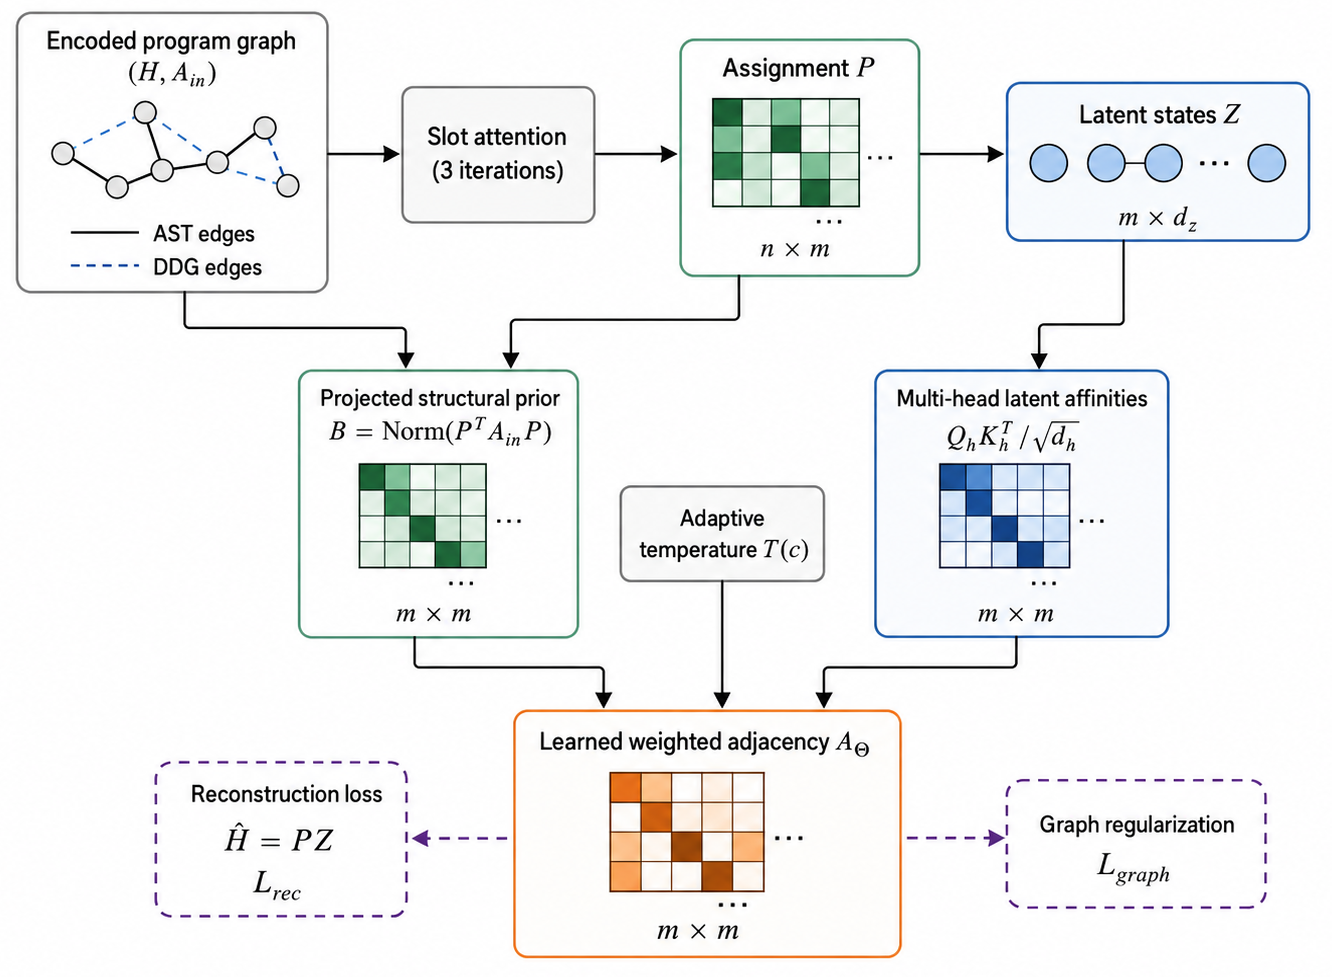
\includegraphics[width=0.96\linewidth]{latent_graph_induction.png}
\caption{Latent graph induction in the original method. Canonical and
node-label lexical inputs are already contained in $H$, so they influence
assignments, latent states, affinities, and the learned adjacency.}
\label{fig:latent}
\end{figure}

\section{Original multi-scale spectral representation}

\subsection{Normalized Laplacian and eigenvalues}

The learned adjacency is sanitized, symmetrized, clipped to $[0,1]$, and stripped
of self-loops. With
\begin{align}
D&=\operatorname{diag}(A_\Theta\mathbf1),\\
L_\Theta&=I-D^{-1/2}A_\Theta D^{-1/2},
\end{align}
the implementation symmetrizes $L_\Theta$ and adds a deterministic diagonal
jitter from $0$ to $10^{-4}$. It computes 32 eigenvalues and clips them to
$[0,2]$.

\textbf{Original gradient behavior.}
In the hybrid implementation, \texttt{eigvalsh} is executed inside
\texttt{torch.no\_grad()}. Density and heat features are therefore numerical
functions of the learned graph at inference, but their gradients do not train the
graph. The differentiable spectral-to-graph path is supplied by the Chebyshev
graph-signal branch described below.

\subsection{Eigenvalue density: 32 features}

For centers $\xi_j$ uniformly spaced on $[0,2]$ and bandwidth $0.08$,
\begin{equation}
d_j(c)=\frac{1}{32}\sum_{i=1}^{32}
\exp\!\left[-\frac12
\left(\frac{\lambda_i-\xi_j}{0.08}\right)^2\right],
\qquad j=1,\ldots,32.
\end{equation}
This is a smooth normalized histogram of the latent graph spectrum.

\subsection{Heat trace: 24 features}

For 24 logarithmically spaced diffusion times
$t_q\in[10^{-2},10^2]$,
\begin{equation}
h_q(c)=\frac{1}{32}\sum_{i=1}^{32}\exp(-t_q\lambda_i),
\qquad q=1,\ldots,24.
\end{equation}
Short times emphasize fine-scale, high-frequency behavior. Long times emphasize
global, low-frequency structure.

\subsection{Chebyshev graph-signal energy: 96 features}

The latent states are projected to eight learned graph signals:
\begin{equation}
X=ZW_s\in\R^{32\times8}.
\end{equation}
Let $\widetilde L=L_\Theta-I$. The Chebyshev recurrence is
\begin{align}
T_0(\widetilde L)X&=X,\\
T_1(\widetilde L)X&=\widetilde L X,\\
T_k(\widetilde L)X
&=2\widetilde L\,T_{k-1}(\widetilde L)X
-T_{k-2}(\widetilde L)X.
\end{align}
Twelve fixed Gaussian-shaped frequency responses are approximated with degree
12 coefficients $c_{bk}$. The filtered signal in band $b$ is
\begin{equation}
F_b=\sum_{k=0}^{12}c_{bk}T_k(\widetilde L)X.
\end{equation}
Band weights are program-dependent:
\begin{equation}
\alpha=\softmax\!\left(W_{\rm band}\LN(\bar z)+b_{\rm band}\right),
\qquad
\bar z=\frac1{32}\sum_{j=1}^{32}z_j.
\end{equation}
For band $b$ and signal $s$,
\begin{equation}
e_{bs}=\alpha_b\,\frac1{32}\sum_{j=1}^{32}F_{bjs}^{\,2}.
\end{equation}
Flattening the $12\times8$ matrix gives 96 energy features. Unlike the detached
eigenvalue features, this branch is differentiable through $L_\Theta$, the learned
adjacency, and latent states.

\subsection{Complete 152-dimensional spectral descriptor}

\begin{equation}
s_\Theta(c)
=d(c)\concat h(c)\concat\operatorname{vec}(e(c))
\in\R^{32+24+96}
=\R^{152}.
\end{equation}
This descriptor is \emph{multi-scale spectral}, but not eigenvalue-only:
its Chebyshev energies depend jointly on the Laplacian and learned latent-node
signals.

\begin{figure}[H]
\centering
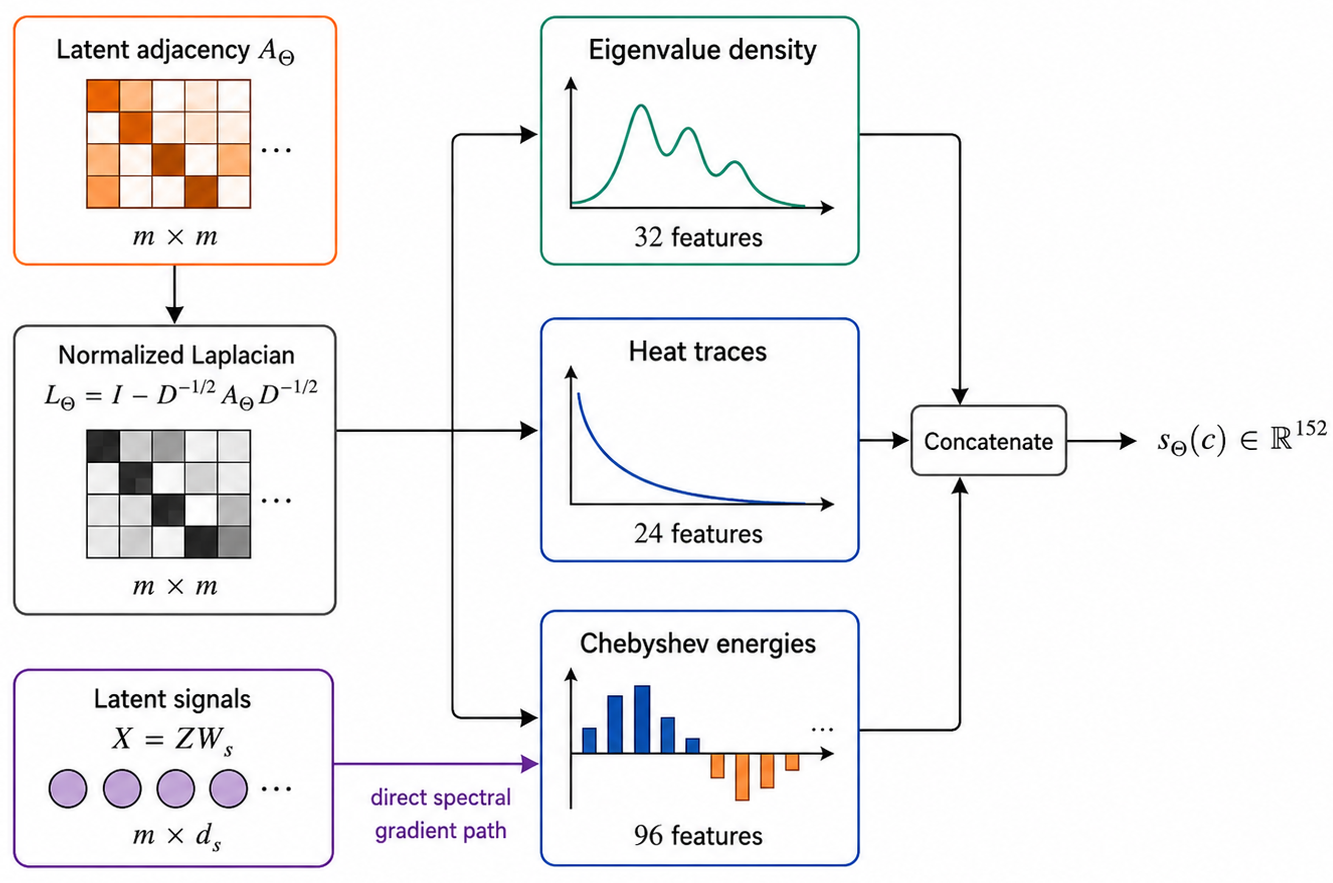
\includegraphics[width=0.94\linewidth]{multiscale_spectral_representation.png}
\caption{The three spectral channels of the original method. Density and heat
traces use eigenvalues; Chebyshev energies use both the Laplacian and learned
signals derived from latent-node states.}
\label{fig:spectrum}
\end{figure}

\section{Hybrid code readout}

\subsection{Spectral projection}

The 152-dimensional descriptor is projected to the common hidden width:
\begin{equation}
z_{\rm spec}
=\GELU\!\left(W_{\rm spec}\LN(s_\Theta)+b_{\rm spec}\right)
\in\R^{256}.
\end{equation}

\subsection{Spectral--latent fusion}

The model separately mean-pools the refined latent-node states:
\begin{equation}
\bar z=\frac1{32}\sum_{j=1}^{32}z_j\in\R^{256}.
\end{equation}
It concatenates this non-spectral vector with the spectral projection:
\begin{align}
u_{\rm hybrid}&=\bar z\concat z_{\rm spec}\in\R^{512},\\
\phi_{\rm graph}
&=\Norm\!\left[
\LN\!\left(
\GELU\!\left(W_{\rm out}\LN(u_{\rm hybrid})+b_{\rm out}\right)
\right)\right]\in\R^{256}.
\end{align}
This is the principal reason the original output is hybrid. Even if density and
heat features were removed or weak, the classifier could still use information
carried directly by $\bar z$.

\subsection{Optional source-lexical residual}

In the lexical-augmented configuration,
\begin{align}
\bar q(c)&=\frac1{96}\sum_{k=1}^{96}E_{\rm lex}(q_k),\\
z_{\rm src}
&=\LN\!\left(
\GELU\!\left(W_{\rm src}\LN(\bar q)+b_{\rm src}\right)
\right),\\
\gamma_{\rm src}&=\sigmoid(g_{\rm src}),\\
\phi(c)&=\Norm\!\left(
\phi_{\rm graph}+\gamma_{\rm src}z_{\rm src}
\right).
\end{align}
$g_{\rm src}$ is initialized to $-0.61903921$, hence
$\gamma_{\rm src}\approx0.35$ initially.

This source-level residual is a direct bypass. It is created from the whole
source text and is added after latent-graph and spectral fusion. Therefore it
does \emph{not} improve the learned graph in the implemented architecture.

\section{Every information and fusion path}

\begin{table}[H]
\centering
\footnotesize
\begin{tabularx}{\linewidth}{@{}p{0.19\linewidth}p{0.24\linewidth}p{0.25\linewidth}X@{}}
\toprule
Fusion point & Inputs & Trainable quantities & Consequence \\
\midrule
Node input fusion & Canonical lookup + gated node-label lexical mean & Two shared embedding tables, lexical gate & Changes $H^{(0)}$ and all downstream graph quantities \\
Relation fusion & Self message + relation-normalized AST/DDG messages & Relation-specific linear maps & Contextualizes input nodes \\
Latent assignment & Contextual nodes + trainable slot states & Q/K/V maps, GRU, MLP, slot seeds & Produces $P$ and program-specific $Z$ \\
Adjacency fusion & Latent affinities + projected observed topology & Q/K maps, prior scale, adaptive temperature & Produces learned $A_\Theta$ \\
Spectral-channel fusion & Density + heat trace + Chebyshev energy & Signal map and band attention; filter bank fixed & Produces 152-D $s_\Theta$ \\
Code fusion & Mean latent state + projected spectral descriptor & Spectral projection and output MLP & Direct non-spectral latent bypass \\
Source residual & Hybrid graph embedding + projected source sketch & Shared lexical table, source projection, source gate & Direct whole-source lexical bypass \\
Pair fusion & Left/right embeddings, difference, product, cosine & Pair-classifier MLP & Produces clone logit \\
\bottomrule
\end{tabularx}
\caption{Complete fusion audit for the original architecture.}
\end{table}

\subsection{Dependency map}

The final lexical-augmented embedding can be written compactly as
\begin{equation}
\phi(c)=\Norm\!\left[
f_{\rm hybrid}\!\left(
\underbrace{\bar Z_\Theta(c)}_{\text{latent path}}
\concat
\underbrace{g_{\rm spec}(s_\Theta(c))}_{\text{spectral path}}
\right)
+\underbrace{\gamma_{\rm src}g_{\rm src}(q(c))}_{\text{direct lexical path}}
\right].
\end{equation}
Both $\bar Z_\Theta$ and $s_\Theta$ depend on canonical categories and node-label
lexical inputs. The source sketch $q(c)$ does not affect graph induction.

\section{Siamese pair classifier}

For $\phi_i=\phi(c_i)$ and $\phi_j=\phi(c_j)$,
\begin{equation}
p_{ij}=
\phi_i\concat\phi_j\concat|\phi_i-\phi_j|
\concat(\phi_i\odot\phi_j)
\concat\cos(\phi_i,\phi_j)
\in\R^{1025}.
\end{equation}
The classifier is
\begin{equation}
o_{ij}=W_2\,
\operatorname{Dropout}_{0.10}
\left[\GELU(W_1p_{ij}+b_1)\right]+b_2,
\end{equation}
with dimensions $1025\rightarrow256\rightarrow1$.

\section{Training objective}

\subsection{Class-weighted binary classification}

The positive-class weight is the training negative/positive ratio, capped at ten:
\begin{equation}
\mathcal L_{\rm cls}
=-\left[w_+y\log\sigmoid(o)
+(1-y)\log(1-\sigmoid(o))\right].
\end{equation}

\subsection{Spectral contrastive term}

Let
\begin{equation}
c_{ij}^{s}
=\cos\!\left(\Norm(s_\Theta(c_i)),\Norm(s_\Theta(c_j))\right).
\end{equation}
The spectral contrastive loss is
\begin{equation}
\mathcal L_{\rm spec}
=\mean_{ij}\left[
y_{ij}(1-c_{ij}^{s})^2
+(1-y_{ij})\max(0,c_{ij}^{s}-0.25)^2
\right].
\end{equation}
Because the original eigenvalues are detached, this term trains graph induction
through the differentiable Chebyshev component, not through density or heat
features.

\subsection{Batch-hard negative term}

For known non-clones, define
\begin{equation}
r_{ij}=\max\!\left(0,\cos(\phi_i,\phi_j)-0.10\right)^2.
\end{equation}
The largest 25\% of $r_{ij}$ values in the batch are averaged as
$\mathcal L_{\rm hard}$.

\subsection{Graph regularization}

The mean off-diagonal density is encouraged toward $0.15$:
\begin{align}
\rho(A_\Theta)
&=\frac{\sum_{b,i\ne j}A_{\Theta,b,ij}}
{N\,m(m-1)},\\
\mathcal L_{\rm dens}&=(\rho(A_\Theta)-0.15)^2.
\end{align}
A connectivity diagnostic/penalty uses the second eigenvalue:
\begin{equation}
\mathcal L_{\rm conn}
=\mean_b\max(0,0.03-\lambda_2^{(b)})^2,
\qquad
\mathcal L_{\rm graph}
=2\mathcal L_{\rm dens}+0.1\mathcal L_{\rm conn}.
\end{equation}
In the original hybrid implementation, $\mathcal L_{\rm conn}$ is computed from
detached eigenvalues and consequently contributes no gradient to graph induction.
The density term remains differentiable.

\subsection{Complete objective}

The configured embedding-level contrastive coefficient is zero. The optimized
objective is therefore
\begin{equation}
\boxed{
\mathcal L
=\mathcal L_{\rm cls}
+0.30\mathcal L_{\rm spec}
+0.20\mathcal L_{\rm hard}
+0.05\mathcal L_{\rm rec}
+0.01\mathcal L_{\rm graph}
}.
\end{equation}
AdamW uses learning rate $10^{-4}$ and weight decay $10^{-4}$. The physical
batch size is 32, gradient accumulation gives an effective batch size of 128,
gradient norm is clipped to one, and validation F1 selects the checkpoint and
decision threshold.

\section{What receives gradient in the original model}

\begin{table}[H]
\centering
\small
\begin{tabularx}{\linewidth}{@{}p{0.27\linewidth}p{0.16\linewidth}X@{}}
\toprule
Path or feature & Differentiable to graph? & Explanation \\
\midrule
Pooled latent state $\bar z$ & Yes & Directly depends on latent refinement, adjacency, slots, graph encoder, and input embeddings \\
Chebyshev energy & Yes & Polynomial graph filters depend on $L_\Theta$ and learned signals $ZW_s$ \\
Eigenvalue density & No in original hybrid & Eigenvalues are computed inside \texttt{no\_grad} \\
Heat trace & No in original hybrid & Same detached eigenvalue path \\
Density regularizer & Yes & Direct function of adjacency values \\
Connectivity penalty & No in original hybrid & Uses detached $\lambda_2$ \\
Node-label lexical input & Yes, indirectly & Enters $H^{(0)}$, then changes $H$, $P$, $Z$, and $A_\Theta$ \\
Source lexical residual & No & Added only after graph/spectral fusion \\
\bottomrule
\end{tabularx}
\caption{Gradient audit of the pre-revision implementation.}
\end{table}

\section{Implemented configurations within the original family}

\begin{table}[H]
\centering
\small
\begin{tabularx}{\linewidth}{@{}lccccX@{}}
\toprule
Configuration & Canonical & Node lexical & Source lexical & Readout & Interpretation \\
\midrule
Topology control & Collapsed & No & No & Hybrid & Structure input, but still latent + spectral output \\
Canonical hybrid & Yes & Yes & No & Hybrid & Original core method \\
Lexical hybrid & Yes & Yes & Yes & Hybrid + residual & Original core plus direct whole-source lexical signal \\
\bottomrule
\end{tabularx}
\caption{The original method family. ``Canonical hybrid'' still includes the
bounded node-label lexical sketch; ``Lexical hybrid'' additionally enables the
96-slot source residual.}
\end{table}

\section{Precise interpretation of the original method}

\subsection{Did lexical and canonical information strengthen the graph?}

\textbf{Node-level canonical and lexical information: yes.}
They formed $H^{(0)}$ before relation-aware message passing and therefore affected
slot assignments, latent-node states, the projected structural prior, learned
affinities, adjacency, Laplacian, and all spectral channels.

\textbf{Whole-source lexical information: no.}
The 96-slot source sketch was projected and added after the hybrid graph embedding
had already been created. It could improve the final score without changing the
learned graph.

\subsection{Was the final representation purely spectral?}

\textbf{No.} It fused:
\begin{enumerate}
\item a 256-dimensional projection of the 152-dimensional spectral descriptor;
\item the 256-dimensional mean of the learned latent-node states;
\item optionally, a 256-dimensional projected source-lexical residual.
\end{enumerate}
Furthermore, 96 of the 152 spectral values were Chebyshev energies constructed
from learned latent-node signals, rather than eigenvalues alone.

\subsection{What did ``node embedding'' mean?}

It could refer to three different quantities:
\begin{enumerate}
\item shared lookup vectors from $E_{\rm can}$ and $E_{\rm lex}$;
\item contextual observed-node states $H$ after relation-aware graph layers;
\item program-specific latent-node states $Z$ produced by slot attention.
\end{enumerate}
The vector used directly in final hybrid fusion was $\bar z=\mean_jz_j$, the pooled
latent-node state. It was not a raw lexical label and not a trainable vector
assigned permanently to each dataset node.

\subsection{Could performance gains be attributed only to the eigenspectrum?}

\textbf{No.} The original architecture intentionally allowed several concurrent
routes. A gain could arise from better graph structure, better Chebyshev
graph-signal features, the direct pooled latent representation, or the optional
source-lexical residual. An ablation was required to attribute gains to a
particular route.

\Needspace{6\baselineskip}
\section{Implementation-aligned forward pass}

\begin{enumerate}[label=\textbf{Step \arabic*:}]
\item Parse source code and export the permitted observed relations.
\item Map raw parser node types to 24 canonical IDs.
\item Produce four stable node-label lexical hash IDs per node.
\item Optionally produce a 96-slot source-token lexical sketch.
\item Retrieve shared canonical and lexical embeddings and construct $H^{(0)}$.
\item Apply two relation-aware graph layers.
\item Apply three slot-attention iterations to obtain $P$ and 32 latent nodes.
\item Project observed AST/DDG topology into latent space as $\widetilde B$.
\item Combine multi-head latent affinity with $\widetilde B$ and adaptive
temperature to obtain $A_\Theta$.
\item Apply two latent graph-refinement layers.
\item Construct the normalized Laplacian.
\item Compute detached eigenvalues, 32 density features, and 24 heat features.
\item Compute eight latent graph signals and 96 attention-weighted Chebyshev
energy features.
\item Concatenate all 152 spectral values and project them to 256 dimensions.
\item Mean-pool the 32 latent states and fuse this vector with the spectral
projection.
\item If enabled, add the projected 96-slot source-lexical residual.
\item Normalize the final code representation.
\item Build the 1025-dimensional pair representation and classify the pair.
\item Optimize classification, spectral, hard-negative, reconstruction, and
graph terms jointly.
\end{enumerate}

\section{Implementation traceability}

\begin{longtable}{@{}p{0.32\linewidth}p{0.61\linewidth}@{}}
\toprule
Method component & Implementation symbol \\
\midrule
\endhead
Configuration and dimensions & \texttt{CanonicalSpectraConfig} \\
Relation-aware input graph & \texttt{RelationGraphLayer} \\
Latent-node induction & \texttt{SlotAttentionInduction} \\
Latent graph refinement & \texttt{LatentGraphRefinement} \\
Spectral channels & \texttt{MultiScaleSpectralExtractor} \\
Hybrid code encoder & \texttt{CanonicalSpectraEncoder} \\
Shared pair model & \texttt{CanonicalSpectraSiam} \\
Training objective & \texttt{canonical\_spectra\_loss} \\
Node-label sketch & \texttt{lexical\_ids} preprocessing path \\
Whole-source sketch & \texttt{source\_lexical\_ids} \\
Original readout switch & \texttt{READOUT\_MODE = "hybrid"} \\
Node lexical switch & \texttt{USE\_NODE\_LEXICAL = True} \\
Source residual switch & \texttt{USE\_SOURCE\_LEXICAL = True} in the lexical configuration \\
\bottomrule
\end{longtable}

\clearpage
\section{Concise methodology statement for a manuscript}

The original \method{} model represented each program as a learned fixed-size
latent graph induced from an observed AST/DDG graph. Canonical node categories
and bounded hashed node-label features were embedded through shared trainable
tables and contextualized using two relation-aware graph layers. Three
slot-attention iterations mapped the variable-size observed graph to 32 latent
nodes. A learned multi-head affinity matrix was fused with an assignment-projected
observed-graph prior and transformed with a complexity-adaptive temperature to
obtain a symmetric weighted latent adjacency. Two further graph layers refined
the latent-node states.

The normalized Laplacian of the learned graph produced a 152-dimensional
multi-scale spectral representation consisting of 32 eigenvalue-density values,
24 heat traces, and 96 attention-weighted Chebyshev graph-signal energies. This
spectral descriptor was projected to 256 dimensions and fused with the mean of
the 32 refined latent-node states. In the lexical-augmented configuration, a
separate 96-slot hashed source-token sketch was projected and added as a gated
residual after this fusion. The resulting normalized code embeddings were
compared by a shared Siamese classifier using the two embeddings, their absolute
difference, elementwise product, and cosine similarity.

\end{document}
